\chapter{\glsentrylongsp{ci}}
\label{ch:sota-ci}

\begin{marginfigure}
	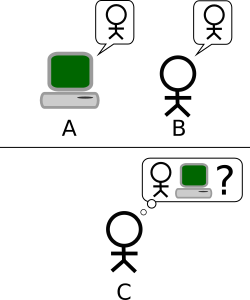
\includegraphics{turing-test}
	\caption{Ilustración del Test de Turing. Modelo propuesto para probar si una máquina es capaz de exhibir comportamiento inteligente similar al del ser humano. Hay tres participantes, dos humanos ($A$ y $C$) y una máquina ($B$), separados entre sí pero pudiendo intercambiarse mensajes de texto. $C$ envía preguntas a $A$ y $B$ sin saber quién es humano y quién es máquina y éstos le responden. Si $C$ no es capaz de identificar qué participante es la máquina, se puede concluir que la máquina es inteligente. Fuente: Hugo Férée, via Wikimedia Commons.}
	\label{fig:turing-test}
\end{marginfigure}

El comportamiento de un individuo en un entorno se ve influenciado por una infinidad de variables. Identificar las relaciones entre éstas es en la mayoría de las ocasiones una tarea que va de lo muy difícil a lo imposible, más aún si añadimos que éstas son muy numerosas y pueden llegar a ser imposibles de cuantificar o incluso de detectar.

La \ac{ci} engloba un conjunto de técnicas que facilitan enormemente estas tareas. En este capítulo se ofrece una perspectiva de la literatura actual sobre las técnicas de la \gls{ci} que son de interés para esta tesis. Introduciremos el concepto y las nociones de \enquote{agente} y de \enquote{aprendizaje} para posteriormente introducir algunas de las técnicas utilizadas dentro del área. Por último, desarrollaremos las tres técnicas principales sobre las que reposa el trabajo teórico de esta tesis: \glsentrylongplsp{ann}, \glsentrylongsp{fl} y \glsentrylongsp{cev}.

\section{\glsentrylongsp{ai} vs. \glsentrylongsp{ci}}

¿Qué es la \ac{ci}? Para entender el significado de éste término tenemos que entender cómo ha evolucionado el término \ac{ai} a lo largo de los años.

El primer concepto a introducir es el de \enquote{conexionismo}. Se puede considerar a Santiago Ramón y Cajal como principal precursor de esta idea por sus trabajos acerca de la estructura de las neuronas y sus conexiónes (e.g. \cite{y1888estructura} y~\cite{ramon1904textura}). Otros prefieren citar el trabajo \textit{\enquote{A logical calculus of the ideas immanent in nervous activity}} (\cite{McCulloch1943}) sobre \glspl{ann} o \textit{\enquote{The organization of behavior}} (\cite{hebb19680}) acerca de la teoría del aprendizaje como primeros trabajos en este tema. Independientemente de su origen, el conexionismo postula que la mente y el conocimiento surgen de redes formadas por unidades sencillas interconectadas (i.e. neuronas).

\begin{marginfigure}
	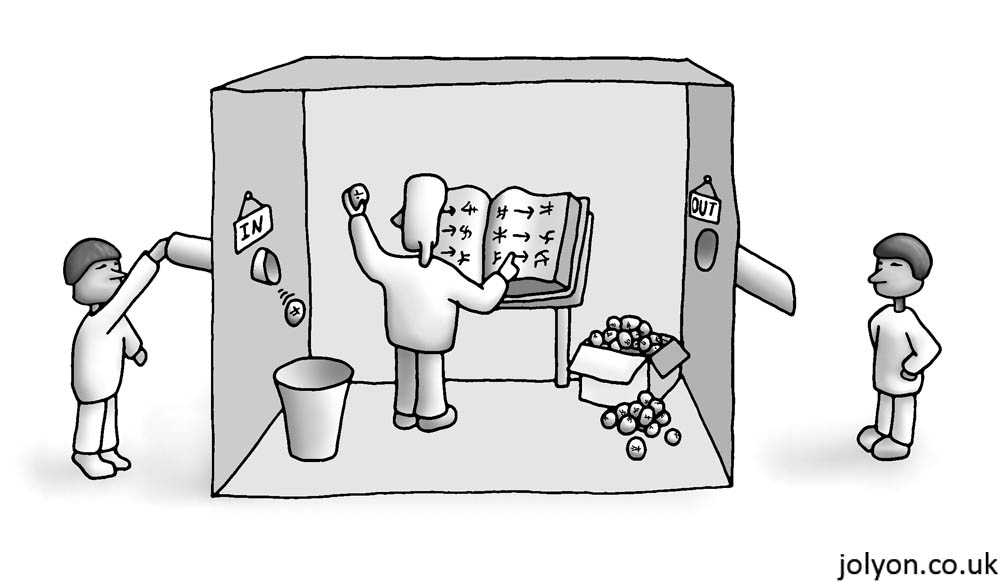
\includegraphics{chinese-room}
	\caption{\enquote{La habitación china} es un experimento mental  propuesto por John Searle que parte de un Test de Turing donde la máquina ha aprendido a hablar chino. Ésta es reemplazada por una persona que no sabe nada del idioma pero que va equipada con manual de correspondencias (ideograma de entrada $\rightarrow$ ideograma de salida). Cuando una persona le manda mensajes en chino, esta otra responde. ¿Podemos decir que dicha persona sabe chino? Evidentemente no. Pero entonces, ¿cómo podemos asegurar que la máquina reemplazada ha \enquote{aprendido} chino?. Autor: Jolyon Troscianko (http://www.jolyon.co.uk/)}
	\label{fig:chinese-room}
\end{marginfigure}

Por otro lado, en 1950, Alan Turing publicó un artículo que comenzaba con la frase \textit{\enquote{Can machines think\sidenote{El propio concepto de \enquote{pensar} es en sí un tema controvertido en el propio ser humano: ¿pensar es algo inherentemente biológico? ¿surge de la mente? Tanto si sí como si no, ¿de qué forma lo hace? Por ello existen detractores de la validez del Test de Turing. Por ejemplo, el experimento de la habitación china (figura~\ref{fig:chinese-room}) nace precisamente como refutación de dicho test, aunque puede llevar a cuestiones quizá más intrigantes. Por ejemplo, si la máquina es capaz de realizar una acción sin entender lo que hace y por qué lo hace, ¿qué garantías tenemos de que el humano sí es capaz? Si los ordenadores operan sobre símbolos sin comprender el verdadero contenido de éstos, ¿hasta qué punto los humanos lo hacen de forma diferente?.}?~\cite{turing1950computing}}}, introduciendo el famoso Test de Turing para determinar si una máquina es o no inteligente (figura~\ref{fig:turing-test}). Se puede considerar este momento como el punto donde se estableció el objetivo a largo plazo del campo de la \ac{ai}, ya que en el artículo Turing propuso un método para determinar si una máquina era capaz de exhibir comportamiento inteligente. Sin embargo, no fue hasta $1956$ en la Conferencia de Dartmouth~\cite{mccarthy1956dartmouth} donde John McCarthy acuñó el término~\ac{ai} a la vez que presentó el tema de la conferencia como la pregunta realizada por Turing en dicho artículo.

A partir de este punto la investigación en~\ac{ai} recibió muchísima atención por parte de investigadores y gobiernos, lo que se tradujo en financiación. Los estudios estaban dominados por aquellos relacionados con las idesa del conexionismo hasta que en $1969$, se publicó el libro \textit{Perceptrons}~\cite{minsky1969perceptrons} de Marvin Minsky y Seymour Papert, donde se expusieron las limitaciones de los modelos de \acp{ann} desarrollados hasta la fecha. El impacto fue tal que la investigación en \gls{ai} se abandonó casi por completo. Concretamente el conexionismo dejó de estar presente en la literatura científica durante dos décadas. Es lo que se conoce como \textit{AI Winter}\sidenote{Es injusto achacar el \textit{AI Winter} sólo al libro \textit{Perceptrons}. El \enquote{efecto gurú} del libro fue sólo la gota que colmó el vaso. A la emoción inicial por los avances le siguieron muchos años de promesas incumplidas, investigación sin resultados significativos, limitaciones de hardware, aumento de la complejidad del software (los comienzos de la crisis del software. Ver~\cite{dijkstra1972humble}). Todo ello provocó un desinterés y una disminución de la financiación que se retroalimentaron la una a la otra.}.

El interés por el campo volvió de nuevo a principios de $1980$ con la aparición en escena de los primeros Sistemas Expertos, los cuales se consideran como el primer caso de éxito en la \gls{ai}  (\cite{russell2003artificial}). A finales de la década, sin embargo, empezaron a resurgir los enfoques conexionistas, en gran parte por la aparición de nuevas técnicas de entrenamiento en perceptrones multicapa o por conceptos como activación no lineal en neuronas (e.g.~\cite{rumelhart1985learning} o~\cite{cybenko1989approximation}). En este momento los sistemas expertos empezaron a perder interés frente al nuevo avance del conexionismo\sidenote{A esta década se la conoce como segundo \textit{AI Winter} dado que la investigación sobre Sistemas Expertos disminuye. Sin embargo no fue un abandono tan acusado como el del primer \textit{AI Winter}.}.

Mientras que el enfoque clásico de la \ac{ai} postulaba que la mente operaba de la misma manera que una máquina de Turing, es decir, mediante operaciones sobre un lenguaje de símbolos, el enfoque del conexionismo postulaba que la mente, el comportamiento inteligente, emergía de modelos a más bajo nivel. Esto provocó que algunas voces se alzaran contra lo que se consideraba el \enquote{enfoque incorrecto} de la \ac{ai}. Sin embargo, otras técnicas alineadas con el conexionismo (debido a su enfoque de comportamiento emergente y aproximación como lo son la \ac{fl} o los \acp{ga}) ganaban popularidad y alimentaban el éxito cosechado por este \enquote{enfoque incorrecto}\sidenote{Es comprensible ya que el método clásico produce modelos fáciles de interpretar mientras que el enfoque conexionista produce modelos cuyo funcionamiento en general no es del todo deducible. Sin embargo, existen problemas con alto grado de complejidad muy difíciles (o imposibles) de modelar. Más aún cuando éstos son de naturaleza estocástica~\cite{siddique2013computational}.}.

Esto provocó una explosión de terminologías para diferenciar las investigaciones de la propia~\ac{ai} clásica. Por un lado se evitaba el conflicto, nombrando lasáreas de trabajo con un término más acorde con el comportamiento o técnica utilizada. Por otro, se separaba de las connotaciones negativas que fue cosechando la \ac{ai} con el paso de los años, \enquote{promesas, pero no resultados}).

Lo verdaderamente interesante es ver la evolución de la literatura, y por tanto de los objetivos de la \ac{ai} durante estos años. En el nacimiento del campo, se buscan literalmente máquinas que piensen como humanos, o al menos seres racionales, con mente. Con el paso de los años (y los continuos choques contra la realidad), la literatura va tendiendo hacia la búsqueda de conductas y comportamientos inteligentes cada vez más específicos. Este hecho se hace más patente en este momento, donde cada investigación se nombra de cualquier forma menos con el término \ac{ai} (e.g \ac{ml}, \acp{rs}, o \ac{nlp}). Es evidente que la \ac{ai} se puede observar desde diferentes puntos de vista, todos perfectamente válidos. En~\cite{russell2003artificial}, tras un análisis de las definiciones existentes en la literatura por parte de diferentes autores, se hace énfasis en este hecho mostrando los diferentes puntos de vista a la hora de hablar de lo que es la \ac{ai}. El resumen se puede observar en la figura~\ref{fig:different-povs-ai}.

\begin{figure}
	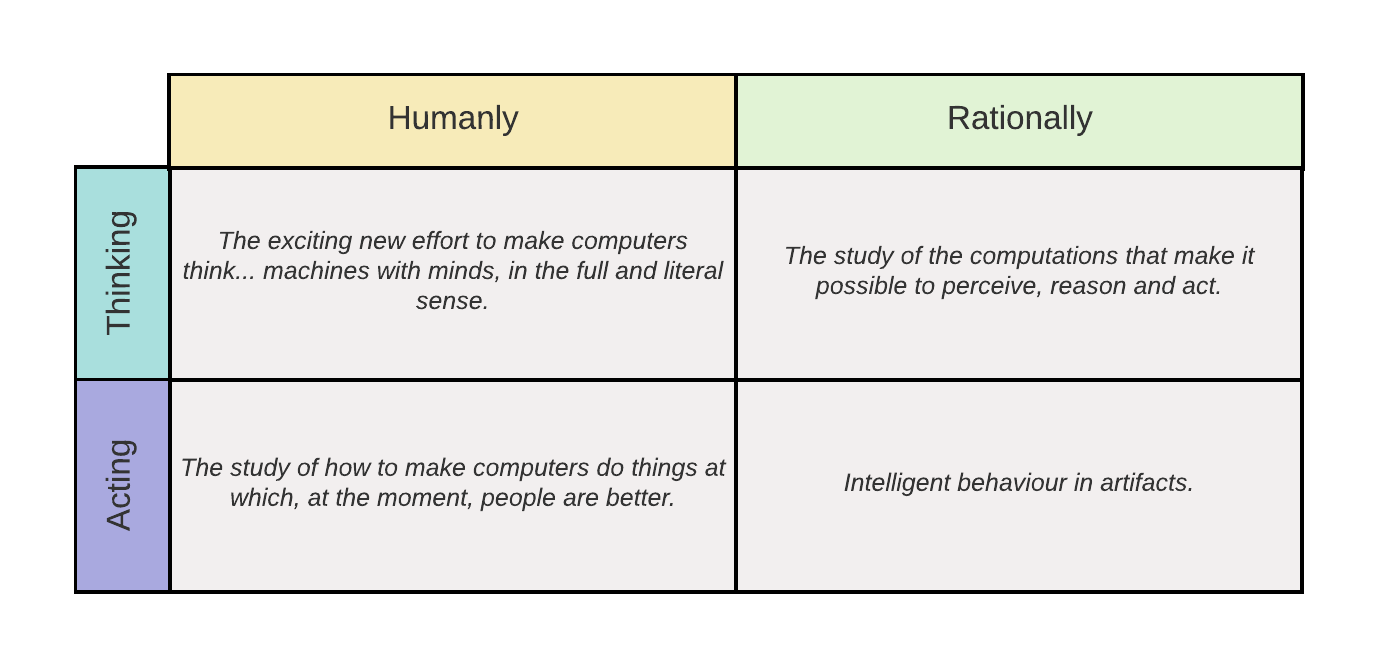
\includegraphics{different-povs-ai}
	\caption{Diferentes objetivos perseguidos por la~\glsentrylongsp{ai}. Las filas diferencian entre pensamiento o comportamiento mientras que las columnas separan entre inteligencia humana o el ideal de la inteligencia (racionalidad). Fuente: \textit{Artificial Intelligence: A Modern Approach ($3^{rd}$ Ed.)},~\cite{russell2003artificial}.}
	\label{fig:different-povs-ai}
\end{figure}

Volviendo al tema de la terminología, muchas de las diferentes técnicas se fueron agrupando dentro de diferentes áreas. Una de ellas es la conocida como \glsentrylong{ci}. Dado que persigue el mismo objetivo a largo plazo y que surje de la propia \ac{ai} parece lógico mantenerla como un subconjunto y no como un nuevo campo del conocimiento humano. Sin embargo, algunos autores abogan por que la \ac{ci} es un campo diferenciado de la \ac{ai}.

Podemos definir la \ac{ci} como la \enquote{\textit{rama de la \ac{ai} que aporta soluciones a \textbf{tareas específicas} de forma \textbf{inteligente} a partir del aprendizaje mediante el uso de \textbf{datos experimentales}}}. A diferencia de la aproximación clásica de la \ac{ai}, se buscan aproximaciones a las soluciones y no las soluciones exactas. Esto es debido a que muchos problemas son de naturaleza compleja, ya sea por la erlación entre sus multiplas variables, a la falta de información o a la imposibilidad de traducirlos a lenguaje binario.

Se puede fijar el año $1994$ como el que el término \ac{ci} nace como área, coincidiendo con el cambio de nombre del \textit{IEEE Neural Networks Council} a \textit{IEEE Computational Intelligence Society} (\url{http://cis.ieee.org/}). Poco antes, en $1993$, Bob Marks en su trabajo~\cite{bezdek1993intelligence} presentó las que él consideraba diferencias fundamentales entre la \ac{ai} y la \ac{ci} resumiéndolas en la siguiente frase.

\blockquote{Neural networks, genetic algorithms, fuzzy systems, evolutionary programming, and artificial life are the building blocks of CI.}

Durante estos años ganaba popularidad también el concepto del \ac{sc}. Éste engloba las técnicas que buscan resolver problemas con información incompleta o con ruido. Debido a que el conjunto de técnicas definidas como consituyentes del \ac{sc} son las mismas que las de la \ac{ci} algunos autores consideran ambos términos equivalentes. Nosotros consideramos que el \ac{sc} es un punto de vista de la computación más que de la \ac{ai} en contraposición con el \ac{hc}, y que la \ac{ci} hace uso de métodos del \ac{sc}\sidenote{El \ac{hc} es como se define la computación convencional frente al \ac{sc}. El \ac{hc} basa sus técnicas en aquellas basadas en modelos analíticos definidos de forma precisa y que en ocasiones requieren mucho tiempo de cómputo. Están basados en lógica binaria, análisis numérico, algoritmos y respuestas exactas. El \ac{sc} por otro lado es tolerante a la imprecisión y al ruido y tiende a llegar a soluciones aproximadas de manera más rápida. Se basa en modelos aproximados, emergencia de algoritmos y modelos estocásticos.}.

\section{Aprendizaje}

La resolución clásica a un problema suele ser la aplicación de una secuencia de instrucciones basadas en un conjunto de símbolos (e.g. una función escrita en el lenguaje de programación C). Esta forma de solucionar un problema no \textit{aprende} a solucionarlo. Se puede interpretar como que la solución está grabada en su memoria.

En la aproximación de la \ac{ci}, existen modelos y existen técnicas para hacer aprender esos modelos. La aplicación de dichas técnicas es lo que se conoce como \textbf{aprendizaje}. Las técnicas de aprendizaje en \ac{ci} se suelen clasificar en $2$ paradigmas:

\begin{itemize}
	\item \textbf{Supervisado}. El entorno presentado al modelo consiste en un conjunto de la forma $D = {(I_i, O_i) | \forall i \in \mathbb{N}}$, donde cada $O_i$ es la salida esperada del modelo a la entrada $I_i$. Los algoritmos tratarán de ajustar el modelo todo lo posible para que las salidas obtenidas sean lo más parecidas a las salidas originales. Este paradigma de entrenamiento suele estar relacionado con problemas de \textit{regresión}.
	\item \textbf{No supervisado}. Al modelo se le ofrece un conjunto de la forma $D = {I_i | \forall i \in \mathbb{N}}$, donde cada $I_i$ es una entrada al problema, pero del que no conocemos la salida. Los algoritmos dentro de esta categoría harán uso de estos datos para ir reajustando el modelo tratando de encontrar las estructuras ocultas entre dichos datos (e.g. patrones, correlaciones o clases). Es un paradigma de entrenamiento íntimamente relacionado con problemas de \textit{clasificación}.
\end{itemize}

Algunos autores hacen uso de técnicas pertenecientes a ambos paradigmas en forma de aproximación híbrida para suplir deficiencias u optimizar/acelerar el aprendizaje. Un claro ejemplo lo podemos ver en \cite{Hinton2006}, donde los autores hacen uso de \textit{autoencoders} como técnica no supervisada para la inicialización de los pesos de una red neuronal y posteriormente realizan un entrenamiento supervisado para la optimización es éstos.

Otros, añaden un paradigma más a estos dos existentes, el denominado aprendizaje \textbf{por refuerzo}. Sin embargo, nosotros preferimos considerarlo como un tipo de aprendizaje supervisado, ya que la única característica que lo diferencia es que es un tipo de aprendizaje que se usa en entornos de aprendizaje \textit{on line} ajustando el modelo en función de los estímulos percibidos del entorno por sus acciones sobre el mismo, y no en un entorno aislado previo de entrenamiento (\textit{off line}), como la práctica totalidad de técnicas supervisadas y no supervisadas.

\section{Técnicas en la \Glsentrylongsp{ci}}

Bajo el paraguas de la \ac{ci} se incluyen muchas técnicas diferentes, entre las cuales están las usadas en esta tesis. El resto de la sección describe el funcionamiento de cada una de estas técnicas.

\subsection{\Glsentrylongplsp{ann}}

Una \acrlongsp{ann} puede considerarse como una herramienta que trata de replicar las funciones cerebrales de un ser vivo de una manera muy fundamental (esto es, desde sus componentes más básicos, las neuronas) basándose para ello en estudios de neurobiología y de ciencia cognitiva moderna del cerebro humano\sidenote{Aún apoyándose en la topología y funcionamiento del cerebro humano para realizar el símil, lo cierto es que dichos modelos distan aún de considerarse \textit{cerebros artificiales}. La red neuronal más compleja hasta la fecha es la propuesta en~\cite{TraskANDREWTRASK}, con alrededor de $160.000$ parámetros a ser ajustados (podemos abstraernos y pensar en ellos como conexiones entre neuronas). Como dato anecdótico, se estima que sólo en el neocórtex (ver figura~\ref{fig:neocortex}) del ser humano existen alrededor de $20.000$ millones de neuronas, cada una de las cuales conectada a entre $100$ y $100.000$ neuronas vecinas (\cite{Pakkenberg1997}). Esto supone entre $2 \cdot 10^{12}$ y $2 \cdot 10^{15}$ conexiones. Tecnológicamente hablando, la sensación esque estamos aún a años luz de aproximarnos siquiera a la complejiadd de un cerebro humano.}.

\begin{figure}
	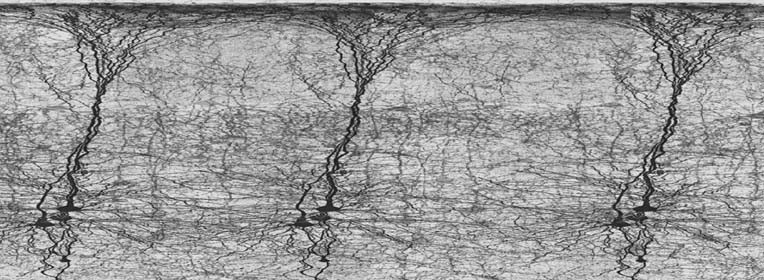
\includegraphics{neocortex}
	\caption{Una sección del neocórtex humano, región asociada a las capacidades cognitivas y que supone alrededor de un $76\%$ del volumen total del cerebro humano. Está distribuído en $6$ capas y miles de columnas que las atraviesan, cada una con alrededor de $10.000$ neuronas y un diámetro de $0.5mm$. Fuente: \textit{Blue Brain Project EPFL}, \url{http://bluebrain.epfl.ch/}.}
	\label{fig:neocortex}
	\setfloatalignment{b}
\end{figure}

Una \ac{ann} es independiente del modelo del problema a solucionar. Se la puede considerar como una caja negra que aprende las relaciones que subyacen en los datos del problema para abstraer el modelo a partir de éstas. Estas características de aprendizaje y abstracción son los factores determinantes por los que son usadas en prácticamente todas las áreas de la ciencia y de la ingeniería (\cite{Du2006}).

\newthought{El modelo de neurona artificial} de McCulloch-Pitts introducido en el trabajo \enquote{A logical calculus of the ideas immanent in nervous activity} (\cite{McCulloch1943}, ilustración en la figura~\ref{fig:mccullocs-pitts-neuron-model}) es el considerado primer trabajo en la disciplina de las \acp{ann}, y aunque existen muchas y muy diferentes tipologías y formas de operar con redes, todas funcionan de la misma manera: unidades (i.e. neuronas) interconectados mediante enlaces por los que fluye la información de manera unidireccional, donde algunas de dichas unidades sirven de entrada al sistema (i.e. entradas o sensores), otras sirven de salida del sistema (i.e. salidas y actuadores) y otras como elementos internos (i.e. ocultas), y donde las conexiones se ajustan mediante un proceso denominado \textit{entrenamiento}.

\begin{figure}
	\missingfigure[figheight=2cm]{Figura del modelo artificial de McCullocs-Pitts}
	\caption{Variación de la representación del modelo de neurona artificial propuesto por McCullocs y Pitts. En éste, cada una de las entradas $x_i$ es incrementada o inhibida aplicando el producto con su peso asociado $w_i$. La activación vendrá determinada por la aplicación de una función (denominada \enquote{de activación}) a la suma de los valores. Esta variación en concreto incluye una entrada $x_0$ y un peso $w_0$ como bias de la neurona para la variación dinámica del umbral de activación.}
	\label{fig:mccullocs-pitts-neuron-model}
\end{figure}

Este primer modelo de neurona proponía una función escalón para determinar si la neurona se activaba o no (analogía al funcoinamiento de la neurona artificial). Posteriormente aparecieron nuevos modelos de neuronas diferentes funciones de activación. De éstas, las más comunes son las de tipo sigmoide\sidenote{
	Concretamente la función logística de pendiente $1$ definida como:
	\begin{equation}
		\frac{1}{1 + e^{-x}}
	\end{equation}
}.

\TODO{Parrafito sobre la limitación de la neurona singular para dar hilo a las topologías}

\newthought{Existen diferentes topologías de redes neuronales} o arquitecturas dependiendo de qué forma toma el grafo que modela las neuronas y sus conexiones. En este caso, las redes neuronales pueden ser de dos tipos:

\begin{itemize}
	\item \textbf{Feed-Forward}. Sus grafos no contienen ninguń ciclo (figura XXX). Es la topología más usada en aplicaciones prácticas debido a su sencillez y su efectividad. En ellas el flujo de información sigue un camino desde las entradas hasta las salidas, sin ninguna retroalimentación. No es requisito que las neuronas se agrupen en capas, aunque suele ser la estructura común. A las redes de más de dos capas ocultas (i.e. las capas que se encuentran entre la capa de neuronas de entrada y la capa de neuronas de salida) se las denomina \enquote{profundas} o \textit{deep}. Algunos tipos pertenecientes a esta categoría pueden ser el Perceptrón [Rosemblat, 1957], el Perceptrón multicapa [Rumelhart et al., 1986], el algoritmo LVQ y su sucesor los Mapas Auto-Organizados [Kohonen, 1998].
	\item \textbf{Recurrentes}. Sus grafos contienen uno o más ciclos, de tal manera que el flujo de información de salida de una neurona puede llegar a afectar a su propio estado. Estas topologías representan de una forma más fiel las bases biológicas de las \ac{ann}, pero son más complejas a la hora de operar y entrenar. Algunos casos particulares de este tipo de arquitectura son las Redes de Hopfield [Hopfield, 1982] o las memorias LSTM (del inglés Long-Short Term Memory) [Hochreiter \& Schmidhuber, 1997].
\end{itemize}

\subsection{Aprendizaje en \glsentrylongplsp{ann}}

\section{\Glsentrylongsp{fl}}

La lógica matemática (y por extensión la teoría de conjuntos)\sidenote{Se puede establecer el siglo IV a.C. como el momento del nacimiento de la lógica dentro de la física Aristotélica, que permaneció inalterada hasta los trabajos de Galileo (cita?) y Newton (cita, seguramente el Principia Matematica) en el siglo XVI. d.C., momento en que se separó y permaneció como disciplina paralela perteneciente más al campo de la filosofía que de la física y la matemática. Empezó a relacionarse de nuevo con la matemática a principios del siglo XIX y a principios del siglo XX la lógica y la teoría de conjuntos pasaron a convertirse en partes indispensables la una de la otra. Por ello suelen ir de la mano cada vez que se habla de la una y de la otra. La evolución de la teoría de conjuntos (Cantor, finales del siglo XIX, buscar referencia) y su unión con la lógica es una época bastante convulsa dentro de la historia de la matemática pero esta tesis no es lugar para su desarrollo. Por ello se ofrece la referencia al libro \textit{La historia de la matemática} de Miguel de Guzmán (referencia. Poner la página. Lo mismo no es de aquí y es del libro de "Los lógicos", pero estoy casi seguro de que es aquí.) en caso de que el lector tenga interés en el tema.} tiene como misión servir de fundamento del razonamiento matemático. Se basa en la definición precisa y con rigor de un razonamiento evitando cualquier tipo de ambigiüedad y de contradicción. Es por ello que la lógica tradicional no suele servir como fundamento de razonamientos del mundo real.

Los conceptos que se manejan en el mundo real suelen ser vagos, llenos de imprecisiones. Además tienden a ser nombrados cualitativamente, no quantitativamente, y cuando existe una correspondencia, ésta suele estar marcada por la subjetividad de los términos.

Explicar lógica difusa y control difuso. Indicar los controladores difusos de segundo, tercer y sucesivos niveles.

\subsection{Teoría de conjuntos difusos}

A diferencia de los conjuntos tradicionales, los conjuntos difusos expresan el grado de pertenencia de un elemento a la categoría representada por el conjunto. La definición podría escribirse de la siguiente manera:

\TODO{Creo que habría que definir antes qué es un dominio}

\begin{definition}
	Sea $X$ una colección de elementos. Se define al \textbf{conjunto difuso} $F$ como un conjunto ordenado de pares de la forma $F = {(x, \mu_F(x)) | x \in X}$, siendo $\mu_F(x) \in [0, 1] \forall x \in X$.
	\label{def:fuzzy-set}
\end{definition}

La función de la definición~\ref{def:fuzzy-set} se denomina \textbf{función de pertenencia}, y caracteriza unívocamente a un conjunto difuso del dominio de $X$.

\TODO{Quizá aquí habría que decir qué es una partición de nu dominio}

\subsection{Operaciones entre conjuntos}

La unión, intersección y el complemento son operaciones básicas en la teoría de conjuntos. \TODO hablar aquí de tnorm, tconorm y complemento, pero someramente. No hay que enrollarse demasiado.

\subsection{Razonamiento}

Al igual que en la lógica tradicional, en la \gls{fl} el razonamiento o inferencia es la manera de extraer conclusiones a partir de premisas en función de un conjunto de reglas.

Estas reglas se expresan como implicaciones, definidas típicamente en lógica difusa como $A \rightarrow B \equiv A \land B$\sidenote{
	Las implicaciones se representan como $A \rightarrow B$, donde $A$ es cualquier operación de premisas y $B$ la conclusión que arrojan.
	
	En lógica tradicional, el valor de verdad de una implicación es equivalente al de la expresión $\not A \lor B$. Sin embargo, en lógicas multivaluadas (y por tanto en lógica difusa) esta equivalencia da lugar a razonamientos que se pueden considerar contraintuitivos.

	En el caso concreto de la lógica difusa se han propuesto gran cantidad de equivalencias. Sólo en los trabajos \cite{Kiszka1985} se analizan $72$ alternativas al operador $\not A \lor B$.
	
	El operador más usado no obstante es el definido como $A \land B$ debido a su rendimiento (en la implicación de Mamdani la $T$-norma se implementa como el operador mínimo).
}.

Las dos formas de extraer conclusiones a partir de premisas en \gls{fl} son el \textit{modus ponens} generalizado (del que hablaremos) y el \textit{modus tollens} generalizado, modificaciones sobre los procesos de inferencia \textit{modus ponens} y \textit{modus tollens}\sidenote{
	En realidad se llaman \textit{modus ponendo ponens} (\enquote{la forma que al afirmar, afirma}) y \textit{modus tollendo tollens} (\enquote{la forma que al negar, niega}).
}, dos formas similares de razonamiento (figura~\ref{fig:modus-ponens-and-modus-tollens}). Nosotros centraremos nuestro discurso en la primera.

\begin{figure}
	\missingfigure[figheight=4cm]{Ilustración con las dos formas de razonamiento}
	\caption{Formas de razonamiento en lógica tradicional: \textit{modus ponendo ponens} y \textit{modus tollendo tollens}.}
	\label{fig:modus-ponens-and-modus-tollens}
\end{figure}

\newthought{El modus ponens generalizado es una generalización del modus ponens de la lógica tradicional} donde, en lugar de expresas las reglas de forma absoluta, se expresan de forma aproximada. En la figura~\ref{fig:modus-ponens-traditional-vs-generalized} se ilustra las diferencias fundamentales entre ambos modos.

\begin{figure}
	\missingfigure[figheight=4cm]{Ilustración con el modus ponens y el modus ponens generalizado}
	\caption{Proceso de razonamiento según el \textit{modus ponens} tradicional frente al \textit{modus ponens} generalizado. En el primero, si la premisa $A$ es cierta, entonces la conclusión $B$ será cierta. En el segundo, dado que la premisa $A$ no es del todo cierta (es $A'$), entonces la conclusión $B$ será cierta sólo en parte ($B'$).}
	\label{fig:modus-ponens-traditional-vs-generalized}
\end{figure}

Para determinar qué grado le asignamos a un consecuente a partir de las premisas parciales y las reglas que dirigen el razonamiento se utiliza un método denominado \textbf{regla composicional de inferencia}.

Una regla $A' \rightarrow B'$ se puede representar como una implicación caracterizada por una función $I(\mu_A(x), \mu_B(y))$ (\cite{Fuller1993}).

\TODO{Explicar mejor porque es terrorífico.}

...

En \cite{Ma2004} hay un capítulo de razonamiento que parece que está guay. Revisarlo un poco a fondo a ver si merece la pena tirar or ahí.

\subsection{\glsentrylong{fis}}

Los \gls{fis} (o \gls{fcs}) son son el caso de éxito de la lógica difusa que más resultados ha cosechado tanto a nivel académico como a nivel industrial. Se trata sistemas que utilizan el razonamiento difuso para inferir una respuesta a partir de un conjunto de entradas.

\begin{figure}
	\missingfigure[figheight=4cm]{Ilustración general de un controlador difuso}
	\caption{Diagrama del esquema general de un \glsentrylong{fis}.}
	\label{fig:fis-general-schema}
\end{figure}

Habitualmente son descritos como un componente dividido en tres bloques conceptuales:

\begin{itemize}
	\item \textbf{Fuzzificación}. Traducir los valores de entrada en crudo del dominio sobre el que está definida cada variable lingüística a sus respectivos grados de pertenencia a conjuntos difusos a través de sus funciones de pertenencia. \TODO Ojo, algunos controladores toman como valores de entrada conjuntos difusos según \cite{Ma2004}. Habrá que buscar sobre ello.
	\item \textbf{Inferencia}. Realiza todo el proceso de razonamiento difuso a partir del conjunto de reglas qeu dan significado a este controlador difuso.
	\item \textbf{Defuzzificación}. Traduce los conjunto difuso resultado del proceso de inferencia a valores del los dominios sobre los que están definidos dichos conjuntos difusos. \TODO En un sugeno, la salida es una función directamente así que se podría especificar que en un tipo Sugeno,se puede ver como que la salida son sólo singletones, manteniendo la generalización del proceso de funcionamiento de un \ac{fis}.
\end{itemize}

Esta división se ilustra en la figura~\ref{fig:fis-general-schema}.

\newthought{Hay varios tipos diferentes de \gls{fis}}, aunque tienden a seguir el esquema básico de un controlador difuso típico (figura~\ref{fig:fis-general-schema}).

\paragraph{Sistemas de tipo Mandamni}

Son la primera aproximación de \gls{fis} propuestos

\paragraph{Sistemas de tipo Takagi-Sugeno}

...

Hablar someramente de los tres tipos clásicos que se usan, e indicar que al final los más usados son el Mandamni y el Sugeno. Añadir también quizá una tabla comparativa enter los tres o al menos entre los dos principales:

El consecuente de un \ac{fis} de tipo Mandamni siempre es un conjunto difuso. Por tanto, el proceso de sacar un valor crisp es costoso. Lo bueno, se mantiene significado semántico de las salidas. El consecuente en un Sugeno es un valor, y se puede decir que no necesita proceso de defuzzificación. Si embargo, la respuesta pierde significado semántico si la suma de la fuerza de salida no es 1 (no entiendo qué quiero decir con esto).

\section{\Glsentrylongsp{cev}}

Otra de las técnicas inspiradas en principios biológicos es la de la \gls{cev}. Esta área de la \gls{ci} trabaja sobre algoritmos iterativos inspirados en la \idx{síntesis evolutiva moderna} o \idx{\textit{neodarwinismo}}.

Existe un conjunto de algoritmos denominados \gls{si} que también son algoritmos iterativos estocásticos inspirados en cómo se comportan sistemas colectivos donde el conocimiento emerge de la interacción de individuos, ya se trate de sistemas naturales como por ejemplo el de las bandadas de murciélagos (\cite{Yang2010}) o de sistemas artificiales como sistemas de partículas abstractas (\cite{Artyukhin2014}). Algunos autores consideran este conjunto de algoritmos como pertenecientes al subcampo de la \gls{cev}, pero nosotros consideramos a la \gls{si} como un subcampo independiente dado que el adjetivo \textit{evolutivo} no es característico de este tipo de algoritmos\sidenote{El punto de vista de los autores que lo incluyen es que la evolución no sólo ha sido la razón de la adaptación de los individuos, sino que también es la causante de comportamientos inteligentes grupales. Y, aunque es una apreciación cierta, el adjetivo \textit{evolutivo} se refiere a cómo trabajan los algoritmos, no a lo que ha propiciado la evolución en la naturaleza.}.

\subsection{\glsentrylongplsp{ga}: bases y funcionamiento}

Un \gls{ga} es un algoritmo iterativo estocástico donde se aplica una serie de pasos inspirados en la \idx{síntesis evolutiva moderna} para la resolución de un problema. Éstos fueron introducidos por John Henry Holland en su libro \textit{\enquote{Adaptation in Natural and Artificial Systems}} (\cite{Holland1975}) y constituyen una familia de soluciones con mucho éxito en problemas de aprendizaje, búsqueda y optimización. Desde nuestro punto de vista, podemos decir que la \gls{cev} es el área que trabaja con \gls{ga}.

\TODO{Esto lo he extraído de una marginnote que no iba bien. Hay que reformular o recolocar}
	Dentro de la \gls{cev} existen familias de algoritmos consideradas por muchos autores como entidades diferentes a los \glspl{ga}:
	
	\begin{itemize}
		\item \textbf{\glspl{es}}. Surgen casi a la par con los \gls{ga} por parte de Ingo Rechenberg (\cite{Rechenberg1973}). Se caracterizan principalmente por ser algoritmos iterativos inspirados en la evolución pero que basan su funcionamiento en los pasos de selección y mutación y donde el reemplazo es total.
		\item \textbf{\gls{gp}}. Sus comienzos se pueden trazar hasta Koza 13, dnode el autro hace usio de algoritmos genético para la generación de programas. La idea de esta aproximación es la de representar los genotipos de los individuos no como cadenas de símbolos (la representación clásica de genotipos) sino como árboles sintácticos.
	\end{itemize}
	
	Quizá en el momento de su nacimiento pudieran estar más diferenciadas, pero en la actualidad se puede pensar en ellas como diferentes especializaciones de un \gls{ga} genérico. En el caso de las \glspl{es}, es evidente que se pueden considerar como una especialización de algoritmo genético donde la recombinación y el reemplazo parcial pasan a un segundo plano, y en el caso de la \gls{gp}, son un \gls{ga} una estructura de datos diferentes para el genotipo (la cual conlleva una serie de modificaciones a los algoritmos de recombinación y mutación, así como una serie de desventajas inherentes a su representación).
\TODO{Hasta aquí}

La \idx{síntesis evolutiva moderna} o \idx{neodarwinismo} es una integración de teorías que complementan la teoría de la evolución propuesta por Charles Darwin. En el momento de enunciar la teoría, no se conocía de qué manera los organismos vivos transmitían sus rasgos característicos a su progenie. Las características en las que se inspiran los \glspl{ga} de la síntesis evolutiva moderna incluyen, entre otras:

\begin{itemize}
	\item El principio de selección natural. Introducido en la teoría de la evolución, el principio de selección natural indica que las características de un individuo en un entorno son las que facilitan (o dificultan) sus posibilidades de reproducción, y por tanto de posibilidad de transmisión de dichas características.
	\item La teoría genética, por Gregor Mendel. Concretamente los conceptos de gen (unidad de información genética que tiene posición y valor dentro de un genotipo), alelo (variación de valor de un gen que da lugar a variaciones en el individuo, como por ejemplo color de ojos), genotipo (conjunto de genes que caracterizan a un individuo de una especie), fenotipo (las características físicas del individuo, determinadas por el genotipo y el entorno) y la herencia genética.
	\item La mutación como fuente de variación dentro de una población.
	\item El principio de diversidad alélica de la genética de poblaciones.
\end{itemize}

\begin{figure}
	\missingfigure[figheight=3.5cm]{Esquema general de funcionamiento de un algoritmo genético}
	\caption{Esquema general del funcionamiento de un \glsentrylong{ga}. Se parte de una población de individuos y en iteraciones de selección-recombinación-mutación-reemplazo se va mejorando la población hasta llegar a una solución que, si bien no tiene por qué ser necesariamente la mejor, es lo suficientemente buena como para ser válida.}
	\label{fig:genetic-algorithm-schema}
\end{figure}

Basándose en estos conceptos, la estructura de un \gls{ga} se asemeja al proceso de evolución de poblaciones finitas de individuos. Un ejemplo de esta estructura lo podemos ver en la figura~\ref{fig:genetic-algorithm-schema} Los principales pasos dentro del algoritmo son los siguientes:

\begin{itemize}
	\item \textbf{Inicialización}. El algoritmo crea una \textit{población} de individuos donde cada uno representa una posible aproximación a la solución del problema a resolver.
	\item \textbf{Selección}. Al igual que en la naturaleza, donde el individuo más apto tiene la mayor probabilidad de sobrevivir y tener descendencia con sus características diferenciadoras, en un \gls{ga} el individuo más apto (que represente una solucion más cercana a la buscada) es el que más probabilidades tiene de ser seleccionado para transmitir sus características a las sucesivas poblaciones.
	\item \textbf{Recombinación}. Tras seleccionar a uno o más individuos, existe una probabilidad (generalmente alta) de que éstos generen uno o más individuos con una composición genética resultado de la combinación de éstos. El algoritmo general habla de selección de $2$ individuos y del operador \enquote{cruce}, pero es posible generalizarlo para que el cruce vaya de $1$ individuo (i.e. no hay cruce, es traspaso de una versión de los genes) a $n$ (i.e. todos los individuos tienen probabilidad de transmitir su genotipo, ya sea directamente o aplicando una función a combinaciones de éstos). La recombinación consigue que la composición genética de los individuos (que probablemente sea buena porque han sido seleccionados frente al resto de individuos) se perpetúe en sucesivas poblaciones.
	\item \textbf{Mutación}. Una vez generada una descendencia en la recombinación (o no, pueden ser los individuos originales), los individuos tiene cierta probabilidad (por lo general baja) de que su genotipo sea modificado aleatoriamente. Esto puede hacer del individuo resultante una mala solución, pero también puede hacer que la solución sea nueva o si no, al menos ofrecer más variedad genética a la población.
	\item \textbf{Reemplazo}. Tras uno o más pasos de selección, recombinación y mutación, los nuevos individuos generados reemplazarán a individuos de la población inicial. En general la población en un \gls{ga} contiene el mismo número de individuos según pasan las generaciones, pero no es un requisito fundamental.
\end{itemize}

\subsection{El balance de la biodiversidad: presión selectiva y convergencia}

Las características de todo individuo vienen determinadas por su genotipo. Éste contiene conjuntos de uno o más genes que se manifiestan en el fenotipo como rasgos característicos del individuo. Algunos rasgos son más favorables que otros\sidenote{Lo bueno o malo que es un individuo viene determinado también por el entorno y no sólo por el individuo. Un ejemplo claro es el de la mariposa del abedul. A principios del siglo XIX, en Inglaterra, la mariposa se confundía con los líquenes de la corteza del abedul debido a que tenían colores y patrones similares (ambas eran blancas). Sin embargo, un cambio en un único gen las convertía en negras, y por tanto muy apetecibles para los depredadores, por lo que se puede concluir que las mejores eran las de color blanco. Sin embargo, para mediados de siglo, el hollín del humo del carbón de las fábricas había teñido de negro la práctica totalidad de los líquenes convirtiendo la ventaja de la mariposa blanca en una total desventaja. Por tanto, los rasgos son favorables dependiendo del entorno.} y hacen que el individuo tenga más probabilidad de sobrevivir y, por tanto, de recombinarse y transmitir sus genes.

\newthought{La presión selectiva} es el mecanismo por el cual se favorece o pensaliza la biodiversidad. Cuando es fácil sobrevivir en un entorno, todas las variaciones de una especie son capaces de recombinarse, tener descendencia y seguir perpetuando rasgos característicos. Cuando es difícil, sólo los más aptos son los que sobreviven y por lo tanto los que se reproducen.

\newthought{La biodiversidad} se refiere a la riqueza genética que existe entre los individuos de la población. Si la biodiversidad es alta, tenemos más posibilidades de combinaciones de genes. Visto de otro modo, cuando tenemos más variedad de genes en la población, la cantidad de posibles soluciones a explorar es mayor.

\begin{figure}
	\missingfigure[figheight=4cm]{Tres gráficas donde se ve el efecto de una biodiversidad muy alta, de una biodiversidad normal y de una biodiversidad muy baja.}
	\caption{No sé cómo explicarlo. uando esté más despierto mejor.}
	\label{fig:different-levels-of-biodiversity}
\end{figure}

Mantener una biodiversidad justa en un \gls{ga} es esencial. Cuando la variedad genética es demasiado baja, los individuos tienden a ser muy parecidos y se hace imposible que aparezcan rasgos genéticos nuevos\sidenote{En realidad sí es posible, con la mutación, pero generalmente es un operador que entra en juego con probabilidad muy baja y por tanto no se puede depender únicamente en él para mantener la biodiversidad.}, haciendo que el algoritmo se estanque. Por otro lado, cuando la variedad genética es muy alta quiere decir que hay muchos individuos todos con características muy distintas. Esto provoca tal cantidad de posibles variaciones que el algoritmo acaba avanzando muy lentamente hacia la solución. Una ilustración de este concepto se puede ver en la figura~\ref{fig:different-levels-of-biodiversity}.

\newthought{Según el algoritmo converge, la biodiversidad disminuye}. Esto es debido a que cuando según vamos acercando nuestra población a una región del espacio, todos los valores que se toman tienden a ser cercanos a esta posición. Esta característica se denomina \textit{explotación}, y es el caso contrario a la \textit{exploración}, es decir, cuando los individuos están distribuidos por todo el espacio de búsqueda buscando posibles soluciones.

Es importante que nuestro algoritmo tienda a explorar en los estacios iniciales de su funcionamiento, y que tienda a explotar cuando se encuentre en momentos cercanos a la localización de una solución. Ésto se puede lograr mediante un buen ajuste de la presión selectiva, aunque el operador de recombinación es el más indicado para gestionar este equilibrio exlporación/explotación.

\subsection{Aptitud y selección de individuos}

Cuando hablamos del individuo \enquote{más apto}, nos referimos a la mejor solución encontrada hasta el momento. Para ello, la manera de decidir cuándo una solución es mejor que otra es la aptitud o \textit{fitness} de una solución.

\newthought{El fitness} de una solución es una función que nos da una idea de la calidad de ésta como número real\sidenote{En realidad, para la mayoría de los algoritmos de los diferentes pasos de un \gls{ga} basta con que la función de fitness defina una función de orden entre soluciones (de la forma \enquote{la solución $S_1$ es mejor que la soución $S_2$}). Sin embargo, asociar un valor real a cada una de las soluciones nos da esta relación de orden además de otras ventajas, como por ejemplo un valor del que podemos observar la evolución a lo largo de los pasos y otros algoritmos como la selección proporcional al fitness.} en su entorno.

El rango del \idx{fitness} depende de la representación de las soluciones y del problema en sí. Una forma muy útil que mantiene la relación de orden y permite su fácil representación gráfica es la mostrada en la ecuación~\ref{eq:fitness-as-error-inverse} (ver figura~\ref{fig:fitness-via-error}). No obstante esta representación es válida únicamente cuando es posible conocer el error de una determinada solución. Otros casos requeriran de funciones alternativas de fitness.

\begin{equation}
	\frac{1}{1 - error}
	\label{eq:fitness-as-error-inverse}
\end{equation}

\begin{figure}
	\missingfigure[figheight=4cm]{Dos gráficas, una donde se ve la evolución del error y otra donde se ve al evolución de su fitness.}
	\caption{Representación del fitness como función inversamente proporcional al error de una solución. Esta forma mantiene el fitness siempre en el intervalo $(0, 1]$. Cuanto menor es el error, esto es, cuanto más tiende a $0$, más se acerca el finess a $1$.}
	\label{fig:fitness-via-error}
\end{figure}

\TODO{No sé si se podría hablar del gaussian kernel aquí cmoo medida del error. De hecho no sé si se usa en algún lado, pero yo creo que sería válido y que da representaciones más fieles en una gráfica.}

\newthought{La selección} se apoya en el fitness para aumentar o disminuir la probabilidad de un individuo para ser seleccionado. Este operador es uno de los más influyentes en un \gls{ga} para mantener el nivel de presión selectiva.

\begin{figure}
	\missingfigure[figheight=4cm]{Tres ilustraciones de cada una de las operaciones de selección bonicas del to.}
	\caption{Tres ilustraciones de las técnicas de selección más comunes en \glsentrylong{ga}. De izquierda a derecha (a) selección proporcional al fitness, (b) selección proporcional a la posición y (c) selección por torneo.}
	\label{fig:selection-techniques}
\end{figure}

El operador de selección se ejecuta cada vez que se quiere seleccionar un individuo para la recombinación por lo que, si la recombinación requiere de dos individuos, el operador de selección será llamado dos veces. Las técnicas más comunes, ilustradas en la figura~\ref{fig:selection-techniques} son las siguientes:

\begin{itemize}
	\item \textbf{Selección proporcional} al fitness (también conocido como \textbf{\idx{selección por torneo}}.). En esta selección a los los individuos se ordenan por fitness y se les asigna una probabilidad proporcional a su fitness. Una vez hecho esto, se genera un valor aleatorio y se comprueba qué individuo ha sido selecciónado. Este operador tiene la desventaja de que, si en un momento unos pocos individuos consiguen un fitness muy alto respecto al resto, acapararán la práctica totalidad del rango de probabilidades, haciendo que disminuya drásticamente la variedad genética.
	\item \textbf{Selección proporcional a la posición}. Varía con el anterior en que la probabilidad asociada a cada individuo es proporcional a la posición y no al fitness. Aunque supone una ventaja respecto al anterior en materia de mantener la biodiversidad, si el tamaño de la población es medio o grande, la probabilidad queda muy repartida, eliminando casi por completo la presión selectiva sobre la población.
	\item \textbf{Selección por torneo}. Esta selección se apoya en dos pasos. En el primero, se extraen aleatoriamente un número $n$ de individuos, independientemente de su \textit{\idx{fitness}}. Una vez extraídos, se seleccionará aquel que tenga el \textit{\idx{fitness}} mayor. Este operador es rápido, dado que no es necesario calcular el fitness de todos los individuos, sino de sólo los seleccionados y, con el parámetro $n$ correctamente seleccionado, mantiene la presión selectiva.
\end{itemize}

\subsection{Representación de individuos}

Un individuo es una solución a nuestro problema. Sin embargo, no existe una única representación para un problema y elegir la mejor representación posible es crucial para un buen desempeño del algoritmo. Para comprender la importancia de una correcta codificación, vamos a formalizar un poco el concepto del problema.

\begin{figure}
	\missingfigure[figheight=4cm]{Lo que pasa cuando las codificaciones van al conjunto de soluciones, fuera del conjunto de soluciones o no exploran todas las soluciones.}
	\caption{Situaciones posibles cuando la cardinalidad del conjunto de las codificaciones de nuestro problema es (a) mayor, (b) menor o (c) igual que la cardinalidad del conjunto del espacio de soluciones posibles.}
	\label{fig:why-we-need-a-correct-codification}
\end{figure}

Supongamos que tenemos $P = {p_1, \ldots, p_n}$ el dominio del problema (determinado por la codificación del problema, es decir, todos los posibles genotipos), $I = {i_1, \ldots, i_m}$ con $m > n$ el dominio de los posibles individuos, $I_v = {i_1, \ldots, i_j} \subset I$ con $m > j$ el subconjunto de $I$ con todos los individuos que son solución y $f:P \rightarrow I$ una aplicación inyectiva (para simplificar nuestra formalización). Dependiendo de la cardinalidad de los conjuntos se nos pueden dar tres casos (figura~\ref{fig:why-we-need-a-correct-codification}):

\begin{enumerate}
	\item $n > j$. Cuando la codificación de nuestro problema genera individuos fuerqa del conjunto de soluciones, quiere decir que habrá codificaciones que nos generen individuos no válidos. Nuestro algoritmo tendrá que tener mecanismos para que estos individuos no sean seleccionados (e.g. asignando un \textit{\idx{fitness}}) de $0$) con la consiguiente penalización en tiempo.
	\item $n < j$. En este caso, todas las codificaciones de nuestras soluciones tendrán una correspondiencia con un individuo válido. Sin embargo, existirán individuos válidos que no serán alcanzados nunca por nuestras codificaciones, y por tanto habrá soluciones no exploradas.
	\item $n = j$. Este caso es el óptimo. Al aplicar $f$ a cualquier codificación de solución para nuestro problema, alcanzaremos un individuo válido. Por tanto no tendremos ningún problema de individuos inválidos ni de soluciones fuera de nuestro alcance.
\end{enumerate}

Por ello es importante dedicar especial atención a la codificación de los genotipos de nuestro individuo. Y aunque la codificación es dependiente del problema, existen codificaciones estándar que se usan en la mayoría de los problemas.

\newthought{La codificación \textbf{en lista}} es quizá la más usada en algoritmos genéticos. En ésta, el genotipo de un individuo se representa como una lista de longitud fija de valores, todos ellos pertenecientes al mismo alfabeto.

Existen dos representantes típicas de esta codificación, dependiendo de si el alfabeto es finito o infinito\sidenote{Esto no quiere decir que sean las únicas, sino que son casi equivalentes. Si, por ejemplo, nuestro problema necesita una codificación donde el alfabeto necesita 16 caracteres, es más eficiente trabajar con un alfabeto hexadecimal. Los alfabetos finitos además tienen una desventaja en función de la cardinalidad del alfabeto: si la cardinalidad es $c$ y la longitud del genotipo es $l$, pueden representar hasta $c^l$ puntos en el espacio por lo que si nuestro problema no requiere de tantos puntos estaremos generando individuos no válidos, con los problemas que ello conlleva (ver~\figurename{fig:why-we-need-a-correct-codification})}: La representación binaria, donde los posibles valores que puede tomar cada gen del genotipo es $0$ o $1$ y la representación real, donde los valores pueden tomar cualquier valor $x \in [0, 1] \subset \mathbb{R}$ (figura~\ref{fig:bin-vs-real-ŕepresentation}).

\begin{figure}
	\missingfigure[figheight=4cm]{Un ejemplo de un problema y una codificacińo de ese problema en binario y en real.}
	\caption{Diferencias entre una representación binaria y una representación real de un problema.}
	\label{fig:bin-vs-real-ŕepresentation}
\end{figure}

No existe una codificación superior a otra, todo depende del problema. El sentido común suele dictar que cuando el dominio del problema es continuo (e.g. aproximación de funciones continuas), se debe usar una codificación infinita mientras que cuando es discreto (e.g. búsqueda de ruta óptima en un grafo), una finita.

\newthought{La codificación en árbol} es otra representación clásica en algoritmos genéticos usada, principalmente, para programación genética. En ella, cada uno de los individuos representa un posible programa. Las ventajas de esta representación son claras: facilidad de definir un problema y longitud variable de genotipos.

Sin embargo, posee dos desventajas principales: la primera es relativa a la operación de recombinación. Debido a que los genes del genotipo son de tipos diferentes (i.e. unos representan a variables, otros representan a constantes, otros a funciones unarias, otros a binarias, ...), es necesario implementar controles para garantizar que un individuo (a) recién creado, (b) resultado de una recombinación o (c) mutado sea válido. La segunda está relacionada con la ventaja de la longitud. Los individuos a lo largo del tiempo en esta representación tienden a crecer (después de todo, el espacio de exploración en un árbol de longitud variable es infinito) por lo que es necsario instalar mecanismos para evitar este comportamiento.

\begin{figure}
	\missingfigure[figheight=4cm]{Un ejemplo de un árbol de programación genética contra un árbol de programación genética guiada por gramáticas.}
	\caption{Diferencias entre un árbol que codifica un programa en \glsentryshort{gp} y uno que codifica una palabra de una gramática libre de contexto en \glsentrylong{gggp}.}
	\label{fig:gp-vs-gggp}
\end{figure}

Una línea muy prometedora con codificaciones en árbol es la de la \gls{gggp}. En ésta los árboles de los inividuos no representan programas en sí, sino una palabra perteneciente a una gramática libre de contexto (figura~\ref{fig:gp-vs-gggp}). De esta manera, se garantiza que la generación de individuos es válida (se generan a partir de unas reglas de producción) y la recombinación y mutación son más sencillas de implementar.

\subsection{Manipulación de individuos: recombinación y mutación}

La población debe evolucionar para llegar a una solución. El principal paso en la evolución de una población en un \gls{ga} es el de la recombinación, y aunque la mutación nos da probabilidad de saltar a regiones del espacio de búsqueda no exploradas con anterioridad, la recombinación guía todo el proceso de búsqueda hacia la solución.

Ambos operadores dependen más de la representación del problema que del problema en sí. Por ello existen operadores genéricos para codificaciones en lista de alfabeto finito o infinito así como para codificaciones de árboles de programa o gramaticales. Esto no quiere decir que estos operadores no se puedan personalizar, sino que son formas de operar con ventajas y desventajas ya conocidas. Por tanto, si es posible codificar un problema de una forma clásica, no es necesario reimplementar los operadores de recombinación y mutación.

\newthought{La recombinación} es la principal responsable de la búsqueda dirigida en el espacio de estados, es decir, de explorar el espacio y explotar las potenciales soluciones. y esta toma dos formas: exploración y explotación. en el espacio guía al algoritmo hacia mejoers soluci

Recombinaciones clásicas para los individuos de antes. Matizar que la recombinación puede depender mucho del problema.

Recombinaciones con árboles y sus problemas principales.

\subsection{Reemplazo de individuos}

Tasa generacional, diferencia entre generacional vs. steady-state y variación de elitismo es en realidad una tasa generacional donde deja un individuo.

Algoritmos de reemplazo clásicos.

\subsection{Variaciones y operadores adicionales}

Hablar de los catastróficos y los que me falten. Hay que encontrar más, porque me parece ridículo un apartado para sólo uno.

\subsection{\glsentrylongpl{ga} distribuidos}

\subsection{Optimización de \glsentrylongpl{fis} mediante \glsentrylongpl{ga}}

\section{Agentes inteligentes}
\label{ch:ci:s:agent-concept}

Si echamos un poco la vista atrás, en la figura~\ref{fig:different-povs-ai} se mostraban los cuatro objetivos perseguidos por la \ac{ai}. En uno de ellos en particular se la entiende como el estudio del conseguir que las entidades (e.g. sistemas, software, \ldots) actúen de la manera más inteligente posible. A dichas entidades se las conoce como \textit{agentes}, concretamente en este contexto como \textit{agentes inteligentes}\sidenote{En realidad los autores prefieren denominarlo \textit{agente racional}, dado que captura la esencia de lo que es un comportamiento inteligente. Sin embargo, según esta definición, hasta un elemento tan rudimentario como un termostato puede ser considerado como elemento inteligente, ya que realiza siempre la mejor acción para cumplir sus objetivos, por simples que puedan parecer. Dónde está el límite entre qué es y que no es un agente inteligente cae dentro de los dominios de la filosofía.}. Sin embargo, si es difícil encontrar un consenso en la definición de agente más lo es a la hora de definir cuándo la conducta de éstos es inteligente.

Lo que sí existe es una serie de características comunes que se repiten a lo largo de la literatura (figura~\ref{fig:agent-properties}):

\begin{itemize}
	\item Operan siempre en un \textbf{entorno}, ya sea éste físico (e.g. una red de carreteras para un vehículo autónomo) o virtual (e.g. un cliente de correo electrónico para un clasificador de spam).
	\item Tienen la capacidad de \textbf{percibir} el entorno por medio de \textit{sensores} y de \textbf{actuar} sobre él por medio de \textit{actuadores}.
	\item Son \textbf{autónomos} en el sentido de que pueden actuar sin intervención externa (e.g. humana u otros agentes) teniendo control sobre su estado interno y su comportamiento. Algunos autores les presuponen una autonomía absoluta mientras que otros hablan de que sólo es necesaria cierta autonomía parcial.
	\item Tienen \textbf{objetivos} a cumplir, actuando para ello sobre el entorno de la manera que les indique su comportamiento.
	\item Pueden ser \textbf{sociales}, es decir, tienen la capacidad de comunicarse con otras entidades (e.g. otros agentes) para llevar a cabo sus objetivos.
\end{itemize}

Por tanto nosotros usaremos la siguiente definición: Un agente es una entidad física o virtual que realiza una acción\sidenote{En \cite{russell2003artificial} se define como \textit{\enquote{\ldots just something that acts}} alegando que la palabra \textit{agent} proviene del latín \textit{agere}. Para clarificar esto, \textit{agere} es la forma verbal para \textit{hacer}, pero imprime un significado de movimiento/actividad diferente que no tiene mucho que ver con \textit{hacer} como forma verbal para \textit{crear} o \textit{dar forma} (de lo que se ocupa el verbo \textit{facere}). Por ello, el verbo \textit{actuar} es un verbo que se relaciona con \textit{agere} y de ahí la definición.} de manera total o parcialmente autónoma dada una secuencia de percepciones del entorno en el que se ubica.

\begin{figure}
	\missingfigure[figheight=3.5cm]{Modelo genérico de agente con sus características típicas}
	\caption{Esquema de un agente y sus propiedades. Aunque no existe una definición comúnmente aceptada de agente, sí que existe una serie de propiedades que los que los identifican. Es autónomo, opera realiza acciones sobre un entorno dependiendo de las percepciones que le llegan de éste y tiene la capacidad de comunicarse con el resto de elementos, incluídos otros agentes.}
	\label{fig:agent-properties}
\end{figure}

Pero, ¿qué hace a un agente inteligente? Según algunos autores, el hecho de que posea unos objetivos y autonomía suficiente para cumplirlos ya denota inteligencia (\TODO{encontrar el trabajo y citar}). Según otros, es necesario que el comportamiento sea flexible, esto es, que sea reactivo (reacciona ante el entorno que percibe), proactivo (iniciativa para tratar de cumplir sus objetivos) y social (capaz de interactuar con otros agentes para cumplir sus objetivos) \cite{Wooldridge1995}. Y otros directamente exigen, además, un comportamiento racional a la hora de cumplir los objetivos para calificarlo de inteligente (\TODO{encontrar el trabajo y citar}).

Por tanto, asumiremos la definición ofrecida por \cite{russell2003artificial} donde, se indica que un agente es considerado \textbf{agente inteligente} cuando éste realiza la mejor acción posible (según un criterio de medida). En este contexto, \enquote{la mejor acción posible} se refiere en términos de objetivos y comprensión del entorno, que puede ser o no correcta\sidenote{Que la comprensión del entorno no sea totales un factor clave que diferencia la racionalidad de la omnisciencia. La omnisciencia significa conocer el resultado de toda acción antes de realizarla y por tanto implica el conocimiento de absolutamente todos los detalles del entorno.La racionalidad existe dentro de un contexto de conocimiento limitado.}.

Las nociones de agentes inteligentes y la de \ac{ci} van de la mano. Esto es debido a que su definición funciona a la perfección para las técnicas de la \ac{ci}, esto es, agentes autónomos que perciben el entorno (problema) y actuan de la mejor manera posible sobre él (resuelven) de acuerdo a su conocimento del medio y su estado interno (en base a algoritmos como \ac{ann}, \ac{fl}, \ldots). Por ello desde mediados de los años 1990 el concepto de agente inteligente ha ganado tanta popularidad\sidenote{Tanto es así que en algunos trabajos se define el objetivo de la \ac{ai} como la implementación de la función agente, esto es, la función que realiza la correspondiencia de una percepción a una acción, para un problema dado.}.

\subsection{Tipos de entorno}

La tupla \textit{(entorno, agente)} es esencialmente una metáfora para referirse a la tupla \textit{(problema, solución)} por lo que existen casi tantos entornos diferentes como problemas.

Afortunadamente es posible caracterizar los entornos de acuerdo a un conjunto de propiedades o dimensiones. Este conjunto es usado por la totalidad de la literatura a la hora de caracterizar entornos:

\begin{itemize}
	\item \textbf{Observable}. Un entorno es \textbf{totalmente observable} cuando el agente es capaz de captar toda la información relevante para la toma de una decisión y no necesita mantener ningún modelo interno del entorno, \textbf{parcialmente observable} cuando la información obtenida es incompleta o tiene ruido y \textbf{no observable} cuando el gente no posee sensores.
	\item \textbf{Multiagente o. monoagente}. Un entorno es \textbf{multiagente} cuando requiere de múltiples agentes interactuando para llegar a una solución mientras que es \textbf{monoagente} cuando sólo requiere de uno para ello.
	\item \textbf{Determinista o. no determinista}. Si el estado del entorno actual depende totalmente del estado anterior, se dice que el entorno es \textbf{determinista}. Si no es así, se considera \textbf{no determinista} o \textbf{estocástico}\sidenote{En general, los entornos del mundo real tienden a ser tan complejos que es imposible para un agente abarcar todos los aspectos medibles de éste. Por lo tanto, sea o no la naturaleza del entorno determinista, en general se suele suponer éste como no determinista.}.
	\item \textbf{Episódico o. secuencial}. Un entorno en el que las acciones se dividen atómicamente donde cada una de ellas conlleva un ciclo de (percepción, decisión, acción) y sin relación una con otra se denomina episódico. Si en lugar de ello la acción del agente puede afectar a las decisiones futuras se dice que el entorno es \textbf{no episódico} o \textbf{secuencial}.
	\item \textbf{Estático o. dinámico}. Si durante la toma de decisioń en entorno no cambia, se dice que el entorno es \textbf{estático}. En caso contrario, se dice que es \textbf{dinámico}.
	\item \textbf{Discreto o. continuo}. Esta dimensión en realidad se divide en cuatro, estado del entorno, tiempo en el entorno, percepciones y acciones. La dimensión es \textbf{discreta} cuando ésta se divide en una partición discretizada, y \textbf{continua} cuando no. Por ejemplo, en el Juego de la Vida de Conway, si se modela en un sistema multiagente, tanto el estado (i.e. tablero) como el tiempo (i.e. turnos) como las percepciones y acciones están discretizadas. Sin embargo, en un entorno de conducción automática se puede determinar que las cuatro dimensiones son continuas.
	\item \textbf{Conocido o. desconocido}. Un entorno es \textbf{conocido} cuando es posible determinar cuál va a ser el resultado de una acción. Si por el contrario no es posible, entonces se dice que es \textbf{desconocido}.
\end{itemize}

\section{Arquitecturas}

Existe una serie de arquitecturas básicas o tipos de agentes que dependen principalmente de cómo perciben el entorno y de qué forma se comportan aunque, dependiendo de los autores, las nomenclaturas, tipologías y esquemas pueden variar. Por ello, hemos decidido ofrecer una abstracción donde poner de manifiesto las partes comunes y no comunes entre arquitecturas.

\begin{figure}
	\missingfigure[figheight=3.5cm]{Arquitectura básica de un agente}
	\caption{Arquitectura básica de un agente. Aunque existen múltiples arquitecturas diferentes, todas se basan en la misma estructura. El agente percibe el entorno, lo interpreta y toma la decisión de cómo actuar sobre él.}
	\label{fig:agent-basic-architecture}
\end{figure}

La figura~\ref{fig:agent-basic-architecture} muestra el esquema de las partes principales de un agente. En general, todo arquitectura de agente inteligente está cortada por el mismo patrón y obedece al siguiente funcionamiento:

\begin{enumerate}
	\item El agente, a través de sus \textbf{sensores}, percibe el entorno en el que éste se mueve.
	\item De acuerdo a cómo recordamos el entorno (llamémoslo \textbf{modelo del entorno}), el agente genera una \textbf{interpretación del entorno} tal y como supone el agente que es. Esto es, percibe el entorno y, de acuerdo a sus sensaciones, lo entiende de una determinada forma.
	\item Esta interpretación del entorno es pasada a un proceso de \textbf{inferencia} el cual, en función la implementación para la consecución de sus objetivos, generará una serie de acciones a realizar sobre el entorno.
	\item Estas acciones serán ejecutadas sobre el entorno a través de una serie de \textbf{actuadores}, provocando probablemente una modificación en éste que será percibida de nuevo en momentos sucesivos.
\end{enumerate}

La primera diferencia clave surge en la manera que se ofrece al bloque de inferencia la interpretación del entorno y genera la primera clasificación (figura~\ref{fig:memory-vs-amnesia-in-agents}):

\begin{figure}
	\missingfigure[figheight=3.5cm]{Arquitectura básica de un agente}
	\caption{Ilustración de la diferencia entre un agente sin modelo de entorno y uno con modelo de entorno. Cada acción realizada por el agente con modelo de entorno tiene en cuenta el estado del entorno en momentos pasados. El agente sin modelo de entorno actúa tal y como interpreta el entorno en cada momento, como si sufriese de amnesia.}
	\label{fig:memory-vs-amnesia-in-agents}
\end{figure}

\begin{itemize}
	\item \textbf{Sin modelo de entorno}. Si el agente ofrece su interpretación del entorno directamente, sin hacer uso de información histórica sobre el entorno que se ha movido. Otras formas de denominar a estos agentes es como \textit{agentes reactivos} o \textit{simple-reflex agents} (\cite{russell2003artificial}). Sin embargo, los términos \textit{reactivo} o \textit{reflex} para algunos autores se refieren a la forma de inducción de acciones a partir de percepciones, y por ello preferimos la denominación \textit{sin modelo de entorno}.
	\item \textbf{Con modelo de entorno}. El agente genera su interpretación más detallada del entorno a partir de las percepciones que llegan desde los sensores y de el histórico del entorno que mantiene. Otras formas de llamarlo es \textit{agentes con estado} o \textit{Model-based}, pero lo hemos denominado de esta manera para diferenciar que el modelo que se mantiene en este punto pertenece únicamente al entorno.
\end{itemize}

\begin{figure}
	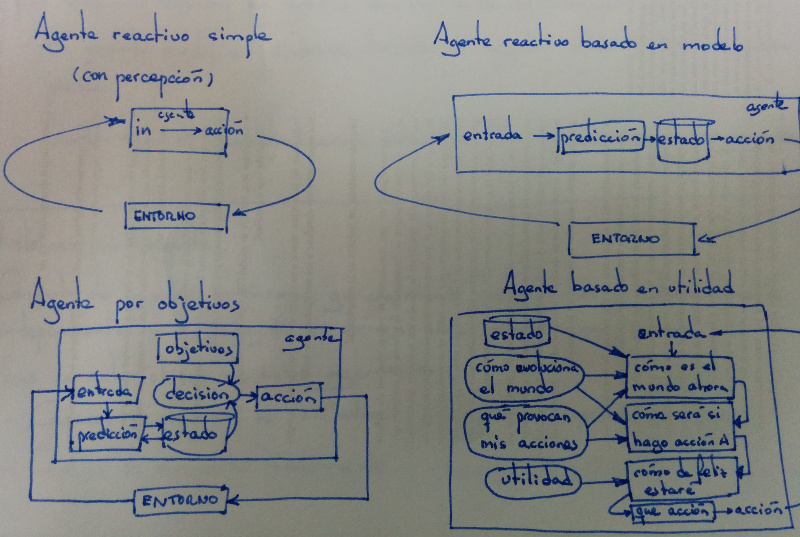
\includegraphics{agent-types}
	\caption{Distintas arquitecturas de agentes en función del comportamiento. Dependiendo de las acciones a realizar, se identifican tres tipos, los reactivos que aplican una acción sin proceso deductivo y los basados en modelo y utilidad (en algunos contextos denominados deliberativos) que basan su comportamiento en alguna forma de deducción.}
	\label{fig:agent-types}
\end{figure}

La siguiente clasificación viene motivada por la forma de deducir el conjunto de acciones a ser aplicadas por parte de los sensores. En este sentido podemos identificar tres tipos distintos de agentes (figura\ref{fig:agent-types}):

\begin{itemize}
	\item \textbf{Reactivos}. Son aquellos donde el uso de un proceso de razonamiento explícito es demasiado costoso para producir una conducta en un tiempo aceptable. Se suelen implementar como correspondencias (percepción $\rightarrow$ acción) sin ningún razonamiento adicional.
	\item \textbf{Basados en objetivos}. Plantean una deducción de forma que determinan cuál sería el estado del entorno tres aplicar varias o todas las acciones que puede realizar. En base a los resultados, selecciona la acción que se corresponde con sus propios objetivos.
	\item \textbf{Basados en utilidad}. Éstos plantean una deducción similar a los basados en objetivos con la diferencia de que, mientras los primeros sólo diferencian entre entorno objetivo o no objetivo, éstos asignan un valor (i.e. \textit{utilidad}) a cada uno de los escenarios de entorno posibles para seleccionar el mejor (e.g. el que mayor utilidad tiene).
\end{itemize}

En la literatura se describen muchos tipos de agente, como por ejemplo los agentes BDI (Believe-Desire-Intention) o los agentes lógicos (i.e. el entorno se representa con reglas lógicas y se infiere mediante métodos como por ejemplo deducción lógica o prueba de teoremas). Sin embargo, éstos pueden definirse en los términos aquí expuestos (figuras~\ref{fig:agent-basic-architecture}, \ref{fig:memory-vs-amnesia-in-agents} y \ref{fig:agent-types}). 

\subsection{\Glsentrylongsp{mas}}

Son aquellos sistemas compuestos de dos o más agentes que interactúan de alguna manera para llegar a una solución.

Cuando los agentes son inteligentes y el problema cae dentro del dominio de la \gls{ai}, el ámbito de estudio es el de la \gls{dai}, la rama dedicada a la resolución de problemas mediante procesamiento descentralizado.

Desde el punto de vista de la ingeniería de sistemas, y a pesar del aumento de complejidad, los \ac{mas}, al ser sistemas inherentemente descentralizados, ofrecen múltiples ventajas frente a los sistemas centralizados tradicionales:

\begin{itemize}
	\item Los sistemas son más robustos y fiables frente a fallos, ya que los agentes son autónomos e independientes del resto.
	\item La modificación del sistema se puede realizar sobre la marcha, agente a agente sin necesidad de parar el sistema al completo.
	\item Su diseño fuerza a desacoplar las dependencias entre agentes.
	\item Son inherentemente paralelizables y por tanto pueden llegar a ser más eficientes que sus homólogos centralizados. Este punto es quizá el más controvertido, ya que esta ganancia en eficiencia se puede perder rápidamente en función de la cantidad de comunicación existente entre agentes.
	\item Debido al nivel de complejidad alcanzado en los sistemas existentes en la actualidad, la computación se distribuye a través de múltiples sistemas, normalmente heterogéneos. La tendencia además es a la alza. La definición de los \ac{mas} hace natural su implementación en este tipo de arquitecturas.
\end{itemize}
	
Desde el punto de vista de la \gls{ai} podemos añadirles la ventaja de que permiten el estudio de conductas complejas de poblaciones a partir del comportamiento de sus elementos básicos, facilitando el estudio de modelosy de teorías sobre éstos.

\newthought{La comunicación entre agentes}, se trata de una característica clave en un \gls{mas}, ya que para denominarse de esta manera dos o más agentes deben interactuar (i.e. comunicarse) entre si. Esta interacción puede implementarse de diversas maneras\sidenote{Las formas clásicas de comunicación son el de paso de mensajes, los sistemas de pizarra y la estigmergia. Para los dos primeros existen dos propuestas para estándar de lenguaje de comunicación, \Ac{kqml} (\cite{Finin1994}) y \Ac{acl} (\cite{Poslad2007}). La tercera forma de comunicación suele ser muy dependiente del problema y no se apoya en lenguajes estándares. Se trata de una forma de comunicación basada en la modificación del entorno, como la efectuada por las hormigas en la búsqueda de alimento, donde éstas dejan rastros de feromonas modificando el entorno para modificar el comportamiento del resto de la colonia.} y siempre toman una o las dos formas siguientes (figura~\ref{fig:communication-between-agents-in-mass}):

\begin{itemize}
	\item \textbf{Cooperación}. Los agentes intercambian información entre sí para llegar a una solución. Esta solución puede ser fragmentada (i.e. cada agente posee parte de la solución y se comunican para ir avanzando de forma común hacia la solución global) o poseerla uno o varios agentes que hacen uso de más agentes para ir avanzando la solución.
	\item \textbf{Competición}. Los agentes compiten dentro de un entorno, generalmente mediante la adquisición de recursos limitados. Un ejemplo de este tipo de sistemas multiagente puede ser aquellos sistemas de vida artificial.
\end{itemize}

\begin{figure}
	\missingfigure[figheight=3.5cm]{Una ilustración de algún entorno de vida artificial donde los agentes compiten y uno de algo donde cooperen}
	\caption{Ilustración de la diferencia entre un agente sin modelo de entorno y uno con modelo de entorno. Cada acción realizada por el agente con modelo de entorno tiene en cuenta el estado del entorno en momentos pasados. El agente sin modelo de entorno actúa tal y como interpreta el entorno en cada momento, como si sufriese de amnesia.}
	\label{fig:communication-between-agents-in-mass}
\end{figure}

\TODO{Aquí una figura de un entorno de vida artificial y un entorno multiagente donde cooperen}
